% The \phantomsection command is needed to create a link to a place in the document that is not a
% figure, equation, table, section, subsection, chapter, etc.
%
% When do I need to invoke \phantomsection?
% https://tex.stackexchange.com/questions/44088/when-do-i-need-to-invoke-phantomsection
\phantomsection

% ---
\chapter{Proposta e implementação de otimização no PSkel-MPPA}
\label{cap:pskelMPPA}
\phantomsection

Com a disponibilização da nova biblioteca de comunicação (\async) pela empresa Kalray para o \mppa, realizou-se o estudo da estrutura e funcionamento da adaptação do \pskelmppa, visando modificações na implementação proposta para fazer uso da nova \api e buscar otimizações anteriormente não exploradas, almejando a melhora do desempenho e de sua eficiência energética.

\section{Implementação com a nova \api de comunicação \async}
\label{sec:implementacao-async}

O fluxo de execução do \pskelmppa continuou semelhante. Durante a fase de inicialização, o processo mestre que está executando no \cluster de \io aloca os dados de entrada e saída na \lpddr, e cria um segmento (conceito da nova \api) específico para cada um deles. Em seguida, ele calcula o número de \tiles alargados que serão produzidos assim como suas dimensões baseado em: i) parâmetros definidos pelo usuário, como o tamanho da entrada de dados e as dimensões do \tile lógico, o número de \clusters de computação e o número de iterações internas; e ii) parâmetros do \kernel estêncil, como o tamanho da máscara. Então, são lançados até 16 processos trabalhadores (um em cada \cluster de computação) e é informado a cada processo trabalhador o número de \tiles alargados gerados, suas dimensões e o subconjunto de \tiles que cada \cluster será responsável por processar, ou seja, ao receber os dados do processo mestre inicialmente o processo trabalhador sabe qual conjunto de \tiles ele será responsável e como deverá computá-lo. Por fim, o processo mestre aguarda até que todos os trabalhadores terminem de computar.
%
Cada processo trabalhador, por outro lado, aloca dados para armazenar os \tiles alargados de entrada e de saída na memória local do \cluster de computação e clona ambos os segmentos de entrada e saída que foram criados pelo processo mestre para realizar futuras transferências de dados. A fase de inicialização tanto do mestre como do trabalhador está encapsulada na classe \texttt{Stencil2D}.
%
Essa primeira etapa do fluxo de execução diferencia-se da anteriormente presente no PSkelMPPA, pois agora esta comunicação é realizada uma única vez na inicialização, o que não ocorria anteriormente, já que existiam trocas de mensagens de sincronização a cada laço da computação iterativa.

A fase de computação consiste da execução do \kernel estêncil pelos processos trabalhadores. As seguintes três principais etapas são realizadas para computar cada \tile atribuído a um processo trabalhador: 1) o \tile alargado é extraído do dado de entrada alocado na \lpddr e transferido para a memória local do \cluster de computação para ser processado; 2) $t^\prime$ iterações do \kernel estêncil (iterações internas) são executadas pelo processo trabalhador sobre o \tile alargado; e 3) o \tile lógico resultante é transferido de volta da memória local do \cluster de computação para a sua posição correspondente na \lpddr. Assim que todos os \tiles atribuídos a cada processo trabalhador forem computados com sucesso, todos os processos trabalhadores irão sincronizar em uma barreira global, pois os processos trabalhadores precisarão dos dados computados pelos outros durante as $t^\prime$ iterações para resolverem as dependências de vizinhança das próximas iterações a serem computadas. 
Foi usada a função \texttt{mppa\_rpc\_barrier\_all()} (proveniente da \api \async) para esse propósito. Todo este processo anteriormente descrito é repetido até que o número total de iterações definido pelo usuário ($t$) seja alcançado.

\begin{figure}[t]
	\centering
	\caption{Comunicações com \texttt{block2d}.}
	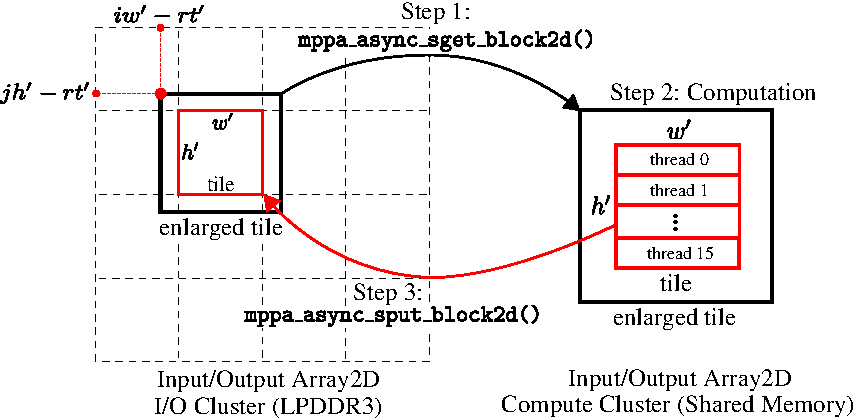
\includegraphics[width=1\textwidth]{figs/pskel-mppa-fluxogram.pdf} \\
  \legend{Fonte: o autor.}
  \label{fig:block2d}
\end{figure}

As etapas acima mencionadas estão retratadas na \autoref{fig:block2d}. Para sua implementação foi utilizada a nova \api de comunicação assíncrona (\async). Abaixo elas são descritas em mais detalhes:

\begin{description}

	\item[Etapa 1.] Baseado na informação fornecida pelo processo mestre durante o processo de lançamento dos \clusters de computação, o processo trabalhador é capaz de calcular as coordenadas de cada \tile alargado atribuído a ele em relação aos dados de entrada alocados na \lpddr (coordenadas $iw^\prime - rt^\prime$ e $jh^\prime - rt^\prime$) sem nenhuma intervenção extra do processo mestre. A função \texttt{mppa\_async\_sget\_block2d()} recebe essa informação e o tamanho do bloco como parâmetros de entrada e ela transfere o \tile alargado para ser processado pelo processo trabalhador do segmento remoto de entrada para a memória local do \cluster de computação através da \noc.

	\item[Etapa 2.] O processo trabalhador computa as $t^\prime$ iterações do \kernel estêncil definido pelo usuário sobre o \tile alargado. Em cada $t^\prime$ iteração, a computação é paralelizada por meio de uma região paralela de OpenMP. A região paralela cria até 16 \threads (uma para cada \pe). Cada \pe é responsável por executar o \kernel estêncil em um subconjunto das células de um \tile alargado, similar a versão com \ipc.

	\item[Etapa 3.] Após a computação do \kernel estêncil, o \tile lógico resultante é transferido de volta para a \lpddr. A função \texttt{mppa\_async\_sput\_block2d()} é usada para esse propósito, permitindo que o \tile lógico seja extraído do \tile alargado na memória local do \cluster de computação e seja transferido para sua posicão correspondente no segmento de saída remoto, sem precisar se preocupar com a criação de portais e o uso do método de \textit{strides}.

\end{description}

\section{Otimização da computação dos elementos de borda da matriz de dados}
\label{sec:otimizacao-bordas}

Ao realizar a computação de elementos próximos às bordas, é feita uma verificação em cada elemento para determinar se ele pertence à borda ou não e tratá-lo conforme necessário. Elementos de computação que beiram a borda física da matriz de entrada precisam acessar os elementos vizinhos, que neste caso são grande parte elementos inacessíveis fisicamente, o que pode acarretar em erros de acesso a memória, como a falha de segmentação. A implementação \ipc realiza no processo de computação esta verificação para cada elemento do \tile presente no \cluster de computação, o que pode degradar seu desempenho. Com isso, pretende-se abordar uma nova maneira de tratamento para os elementos do \tile que beiram a borda da matriz de dados. 

\begin{figure}[b]
  \begin{lstlisting}[
      caption={Trecho de código que define a área de trabalho.}, 
      label=code:workarea,
      language=C++,
      keywordstyle=\color{blue}\bfseries,
      otherkeywords = {__parallel__,struct,Array2D,Stencil2D}, 
      basicstyle=\tiny, 
      frame = single,]
struct work_area_t {
int x_init,  /* X inicial da área de trabalho */
    y_init,  /* Y inicial da área de trabalho */
    x_final, /* X final da área de trabalho */
    y_final; /* Y final da área de trabalho */
    std::vector<int> dist_to_border; /* Vetor que define as distâncias entre os elementos mais externos e as bordas */
};
  \end{lstlisting}
\end{figure}

A ideia é definir uma área de trabalho para cada \tile que será computado e gerenciar essa área ao longo das iterações, reduzindo significativamente o número de verificações que ocorre em cada elemento do \tile e em cada iteração. Na abordagem proposta neste TCC, o \cluster já possui as coordenadas sobre as quais ele deve realizar sua computação, sem precisar verificar elemento por elemento. No caso dos \tiles localizados centralmente na matriz sem contato com a borda, esta área de trabalho seria a máxima possível sem sofrer restrições.
Esta área de trabalho é definida por uma \textit{struct}, que é um tipo de dado composto na qual uma lista de variáveis podem ser declaradas para mais tarde serem acessadas através de um ponteiro único para cada uma. O \autoref{code:workarea} apresenta esta estrutura, e a \autoref{fig:workarea} ilustra seu uso.

Nesta estrutura são definias duas coordenadas, \texttt{(x\_init, y\_init)} e \texttt{(x\_final,y\_final)} que delimitam a área de trabalho. O vetor \texttt{dist\_to\_border} contém a distância entre os elementos mais externos e as bordas da matriz de dados, e com base nesses valores define os deslocamentos necessários a serem aplicados às coordenadas que delimitam a área de trabalho. Todos esses cálculos e definições encontram-se encapsulados dentro do \textit{back-end} do \pskelmppa \async, o desenvolvedor que faz uso do \fw não precisa lidar com estes detalhes. 

\begin{figure}
  \centering
  \caption{Ilustração área de trabalho (\textit{struct work\_area}).}
  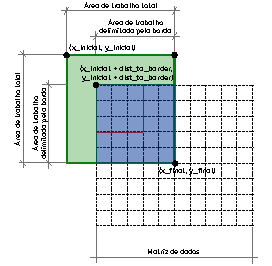
\includegraphics[width=0.8\textwidth]{figs/work_area.pdf}
  \legend{Fonte: o autor.}
  \label{fig:workarea}
\end{figure}

